\documentclass{standalone}
\usepackage{tikz}
\usetikzlibrary{patterns}
\usetikzlibrary{positioning}
\usetikzlibrary{patterns, positioning}
\usetikzlibrary{shapes.misc}
\usepackage[outline]{contour}
\contourlength{1.5pt} 
\usetikzlibrary{calc}
        \usepackage{relsize}
        \tikzset{fontscale/.style = {font=\relsize{#1}}}

\begin{document}
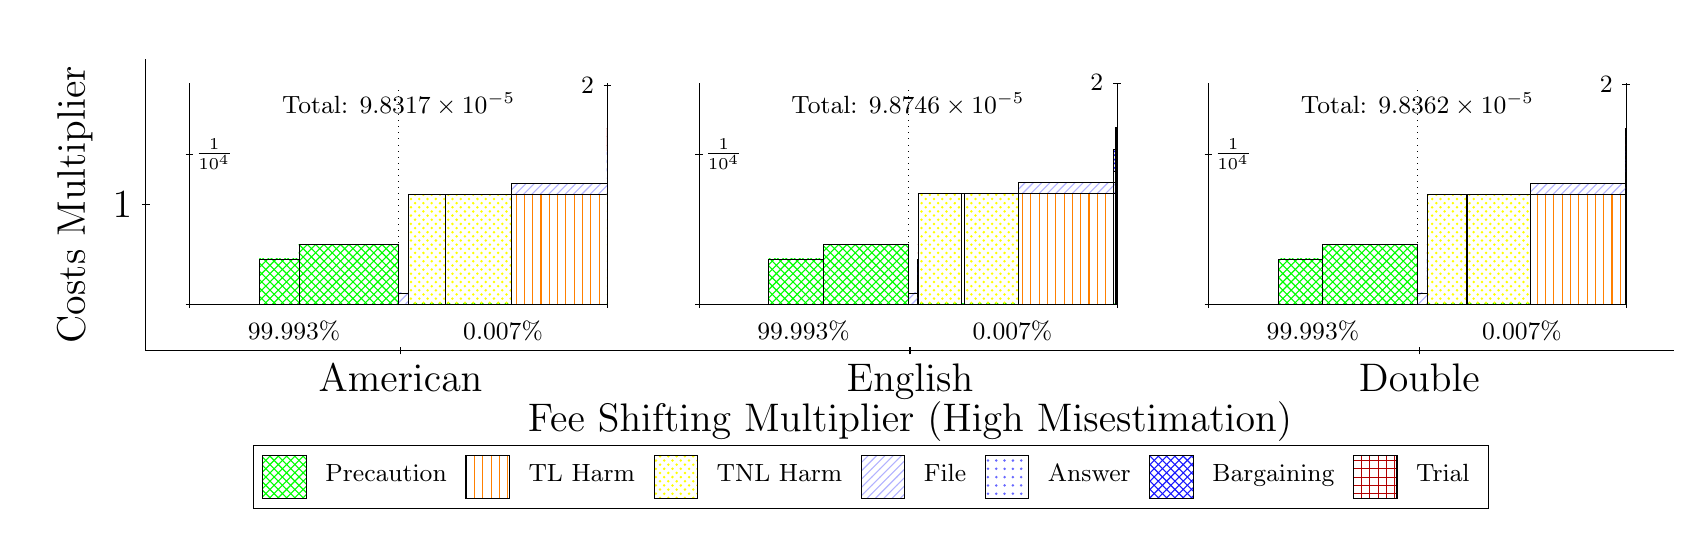
\begin{tikzpicture}
\clip(-0.5,-1.1) rectangle +(20.91,6.2);
\draw[black] (1,1) -- (1,4.7);
\node[rotate=90, fontscale=2, anchor=center] at (0.1, 2.85) {Costs Multiplier};
\draw[black] (0.95,2.85) -- (1.05,2.85);
\node[fontscale=2, anchor=east] at (0.95, 2.85) {1};

\draw[black] (1,1) -- (20.41,1);
\node[fontscale=2, anchor=center] at (10.705, 0.1) {Fee Shifting Multiplier (High Misestimation)};
\draw[black] (4.235,0.95) -- (4.235,1.05);
\node[fontscale=2, anchor=north] at (4.235, 0.95) {American};
\draw[black] (10.705,0.95) -- (10.705,1.05);
\node[fontscale=2, anchor=north] at (10.705, 0.95) {English};
\draw[black] (17.175,0.95) -- (17.175,1.05);
\node[fontscale=2, anchor=north] at (17.175, 0.95) {Double};


\draw[pattern=crosshatch, pattern color=green,draw=black,very thin] (2.4404,1.592) rectangle (2.943,2.1624);
\draw[pattern=crosshatch, pattern color=green,draw=black,very thin] (2.943,1.592) rectangle (4.21,2.3526);
\draw[pattern=north east lines, pattern color=blue!30,draw=black,very thin] (4.21,1.592) rectangle (4.331,1.731);
\draw[pattern=crosshatch, pattern color=green,draw=black,very thin] (4.331,1.592) rectangle (4.3323,1.592);
\draw[pattern=north east lines, pattern color=blue!30,draw=black,very thin] (4.331,1.592) rectangle (4.3323,1.7311);
\draw[pattern=dots,  pattern color=blue!60,draw=black,very thin] (4.331,1.7311) rectangle (4.3323,1.8701);
\draw[pattern=crosshatch,      pattern color=blue!90,draw=black,very thin] (4.331,1.8701) rectangle (4.3323,2.1481);
\draw[pattern=grid,            pattern color=red!70!black,draw=black,very thin] (4.331,2.1481) rectangle (4.3323,2.4261);
\draw[pattern=crosshatch, pattern color=green,draw=black,very thin] (4.3323,1.592) rectangle (4.7979,1.592);
\draw[pattern=crosshatch dots, pattern color=yellow,draw=black,very thin] (4.3323,1.592) rectangle (4.7979,2.9822);
\draw[pattern=crosshatch, pattern color=green,draw=black,very thin] (4.7979,1.592) rectangle (4.8061,1.592);
\draw[pattern=vertical lines, pattern color=orange,draw=black,very thin] (4.7979,1.592) rectangle (4.8061,2.9822);
\draw[pattern=crosshatch, pattern color=green,draw=black,very thin] (4.8061,1.592) rectangle (5.6466,1.5921);
\draw[pattern=crosshatch dots, pattern color=yellow,draw=black,very thin] (4.8061,1.5921) rectangle (5.6466,2.9822);
\draw[pattern=vertical lines, pattern color=orange,draw=black,very thin] (5.6466,1.592) rectangle (6.8569,2.9821);
\draw[pattern=north east lines, pattern color=blue!30,draw=black,very thin] (5.6466,2.9821) rectangle (6.8569,3.1211);
\draw[pattern=crosshatch, pattern color=green,draw=black,very thin] (6.8569,1.592) rectangle (6.8609,1.592);
\draw[pattern=crosshatch dots, pattern color=yellow,draw=black,very thin] (6.8569,1.592) rectangle (6.8609,2.9822);
\draw[pattern=north east lines, pattern color=blue!30,draw=black,very thin] (6.8569,2.9822) rectangle (6.8609,3.1212);
\draw[pattern=dots,  pattern color=blue!60,draw=black,very thin] (6.8569,3.1212) rectangle (6.8609,3.2602);
\draw[pattern=crosshatch,      pattern color=blue!90,draw=black,very thin] (6.8569,3.2602) rectangle (6.8609,3.5382);
\draw[pattern=grid,            pattern color=red!70!black,draw=black,very thin] (6.8569,3.5382) rectangle (6.8609,3.8162);
\draw[pattern=crosshatch, pattern color=green,draw=black,very thin] (6.8609,1.592) rectangle (6.8644,1.592);
\draw[pattern=vertical lines, pattern color=orange,draw=black,very thin] (6.8609,1.592) rectangle (6.8644,2.9822);
\draw[pattern=north east lines, pattern color=blue!30,draw=black,very thin] (6.8609,2.9822) rectangle (6.8644,3.1212);
\draw[pattern=dots,  pattern color=blue!60,draw=black,very thin] (6.8609,3.1212) rectangle (6.8644,3.2602);
\draw[pattern=crosshatch,      pattern color=blue!90,draw=black,very thin] (6.8609,3.2602) rectangle (6.8644,3.5382);
\draw[pattern=grid,            pattern color=red!70!black,draw=black,very thin] (6.8609,3.5382) rectangle (6.8644,3.8162);
\node[font=\small,text=black,anchor=north] at (4.21, 4.4) {Total: $9.8317\times 10^{-5}$};
\draw[black,very thin] (1.5556,1.592) -- (1.5556,4.4);
\draw[black,very thin] (1.5056,1.592) -- (1.6056,1.592);
\node[font=\small,text=black, anchor=west] at (1.5056, 1.592) {};
\draw[black,very thin] (1.5056,3.4935) -- (1.6056,3.4935);
\node[font=\small,text=black, anchor=west] at (1.5056, 3.4935) {$\frac{1}{10^{4}}$};

\draw[black,dotted,very thin] (4.21,1.6762) -- (4.21,4.3158);
\draw[black,very thin] (6.8644,1.592) -- (6.8644,4.4);
\draw[black,very thin] (6.8144,4.3722) -- (6.9144,4.3722);
\node[font=\small,text=black, anchor=east] at (6.8144, 4.3722) {\contour{white}{2}};

\draw[black,very thin] (1.5556,1.592) -- (6.8644,1.592);
\draw[black,very thin] (1.5556,1.542) -- (1.5556,1.642);
\node[font=\small,text=black, anchor=north] at (1.5556, 1.542) {};
\draw[black,very thin] (6.8644,1.542) -- (6.8644,1.642);
\node[font=\small,text=black, anchor=north] at (6.8644, 1.542) {};

\node[font=\small,text=black,anchor=south] at (2.8828, 0.992) {99.993\%};
\node[font=\small,text=black,anchor=south] at (5.5372, 0.992) {0.007\%};

\draw[pattern=crosshatch, pattern color=green,draw=black,very thin] (8.9104,1.592) rectangle (9.6043,2.1624);
\draw[pattern=crosshatch, pattern color=green,draw=black,very thin] (9.6043,1.592) rectangle (10.68,2.3526);
\draw[pattern=north east lines, pattern color=blue!30,draw=black,very thin] (10.68,1.592) rectangle (10.8,1.7324);
\draw[pattern=crosshatch, pattern color=green,draw=black,very thin] (10.8,1.592) rectangle (10.806,1.592);
\draw[pattern=north east lines, pattern color=blue!30,draw=black,very thin] (10.8,1.592) rectangle (10.806,1.7324);
\draw[pattern=dots,  pattern color=blue!60,draw=black,very thin] (10.8,1.7324) rectangle (10.806,1.8728);
\draw[pattern=crosshatch,      pattern color=blue!90,draw=black,very thin] (10.8,1.8728) rectangle (10.806,2.1536);
\draw[pattern=crosshatch, pattern color=green,draw=black,very thin] (10.806,1.592) rectangle (10.809,1.592);
\draw[pattern=north east lines, pattern color=blue!30,draw=black,very thin] (10.806,1.592) rectangle (10.809,1.7324);
\draw[pattern=dots,  pattern color=blue!60,draw=black,very thin] (10.806,1.7324) rectangle (10.809,1.8728);
\draw[pattern=crosshatch,      pattern color=blue!90,draw=black,very thin] (10.806,1.8728) rectangle (10.809,2.1536);
\draw[pattern=grid,            pattern color=red!70!black,draw=black,very thin] (10.806,2.1536) rectangle (10.809,2.4344);
\draw[pattern=crosshatch, pattern color=green,draw=black,very thin] (10.809,1.592) rectangle (11.361,1.592);
\draw[pattern=crosshatch dots, pattern color=yellow,draw=black,very thin] (10.809,1.592) rectangle (11.361,2.996);
\draw[pattern=crosshatch, pattern color=green,draw=black,very thin] (11.361,1.592) rectangle (11.392,1.592);
\draw[pattern=vertical lines, pattern color=orange,draw=black,very thin] (11.361,1.592) rectangle (11.392,2.996);
\draw[pattern=crosshatch, pattern color=green,draw=black,very thin] (11.392,1.592) rectangle (12.086,1.5921);
\draw[pattern=crosshatch dots, pattern color=yellow,draw=black,very thin] (11.392,1.5921) rectangle (12.086,2.996);
\draw[pattern=vertical lines, pattern color=orange,draw=black,very thin] (12.086,1.592) rectangle (13.284,2.996);
\draw[pattern=north east lines, pattern color=blue!30,draw=black,very thin] (12.086,2.996) rectangle (13.284,3.1364);
\draw[pattern=crosshatch, pattern color=green,draw=black,very thin] (13.284,1.592) rectangle (13.293,1.592);
\draw[pattern=crosshatch dots, pattern color=yellow,draw=black,very thin] (13.284,1.592) rectangle (13.293,2.996);
\draw[pattern=north east lines, pattern color=blue!30,draw=black,very thin] (13.284,2.996) rectangle (13.293,3.1364);
\draw[pattern=dots,  pattern color=blue!60,draw=black,very thin] (13.284,3.1364) rectangle (13.293,3.2768);
\draw[pattern=crosshatch,      pattern color=blue!90,draw=black,very thin] (13.284,3.2768) rectangle (13.293,3.5576);
\draw[pattern=crosshatch, pattern color=green,draw=black,very thin] (13.293,1.592) rectangle (13.315,1.592);
\draw[pattern=vertical lines, pattern color=orange,draw=black,very thin] (13.293,1.592) rectangle (13.315,2.996);
\draw[pattern=north east lines, pattern color=blue!30,draw=black,very thin] (13.293,2.996) rectangle (13.315,3.1364);
\draw[pattern=dots,  pattern color=blue!60,draw=black,very thin] (13.293,3.1364) rectangle (13.315,3.2768);
\draw[pattern=crosshatch,      pattern color=blue!90,draw=black,very thin] (13.293,3.2768) rectangle (13.315,3.5576);
\draw[pattern=crosshatch, pattern color=green,draw=black,very thin] (13.315,1.592) rectangle (13.329,1.592);
\draw[pattern=crosshatch dots, pattern color=yellow,draw=black,very thin] (13.315,1.592) rectangle (13.329,2.996);
\draw[pattern=north east lines, pattern color=blue!30,draw=black,very thin] (13.315,2.996) rectangle (13.329,3.1364);
\draw[pattern=dots,  pattern color=blue!60,draw=black,very thin] (13.315,3.1364) rectangle (13.329,3.2768);
\draw[pattern=crosshatch,      pattern color=blue!90,draw=black,very thin] (13.315,3.2768) rectangle (13.329,3.5576);
\draw[pattern=grid,            pattern color=red!70!black,draw=black,very thin] (13.315,3.5576) rectangle (13.329,3.8384);
\draw[pattern=crosshatch, pattern color=green,draw=black,very thin] (13.329,1.592) rectangle (13.334,1.592);
\draw[pattern=vertical lines, pattern color=orange,draw=black,very thin] (13.329,1.592) rectangle (13.334,2.996);
\draw[pattern=north east lines, pattern color=blue!30,draw=black,very thin] (13.329,2.996) rectangle (13.334,3.1364);
\draw[pattern=dots,  pattern color=blue!60,draw=black,very thin] (13.329,3.1364) rectangle (13.334,3.2768);
\draw[pattern=crosshatch,      pattern color=blue!90,draw=black,very thin] (13.329,3.2768) rectangle (13.334,3.5576);
\draw[pattern=grid,            pattern color=red!70!black,draw=black,very thin] (13.329,3.5576) rectangle (13.334,3.8384);
\node[font=\small,text=black,anchor=north] at (10.68, 4.4) {Total: $9.8746\times 10^{-5}$};
\draw[black,very thin] (8.0256,1.592) -- (8.0256,4.4);
\draw[black,very thin] (7.9756,1.592) -- (8.0756,1.592);
\node[font=\small,text=black, anchor=west] at (7.9756, 1.592) {};
\draw[black,very thin] (7.9756,3.4935) -- (8.0756,3.4935);
\node[font=\small,text=black, anchor=west] at (7.9756, 3.4935) {$\frac{1}{10^{4}}$};

\draw[black,dotted,very thin] (10.68,1.6762) -- (10.68,4.3158);
\draw[black,very thin] (13.334,1.592) -- (13.334,4.4);
\draw[black,very thin] (13.284,4.3999) -- (13.384,4.3999);
\node[font=\small,text=black, anchor=east] at (13.284, 4.3999) {\contour{white}{2}};

\draw[black,very thin] (8.0256,1.592) -- (13.334,1.592);
\draw[black,very thin] (8.0256,1.542) -- (8.0256,1.642);
\node[font=\small,text=black, anchor=north] at (8.0256, 1.542) {};
\draw[black,very thin] (13.334,1.542) -- (13.334,1.642);
\node[font=\small,text=black, anchor=north] at (13.334, 1.542) {};

\node[font=\small,text=black,anchor=south] at (9.3528, 0.992) {99.993\%};
\node[font=\small,text=black,anchor=south] at (12.007, 0.992) {0.007\%};

\draw[pattern=crosshatch, pattern color=green,draw=black,very thin] (15.38,1.592) rectangle (15.943,2.1624);
\draw[pattern=crosshatch, pattern color=green,draw=black,very thin] (15.943,1.592) rectangle (17.15,2.3526);
\draw[pattern=north east lines, pattern color=blue!30,draw=black,very thin] (17.15,1.592) rectangle (17.271,1.7314);
\draw[pattern=crosshatch, pattern color=green,draw=black,very thin] (17.271,1.592) rectangle (17.273,1.592);
\draw[pattern=north east lines, pattern color=blue!30,draw=black,very thin] (17.271,1.592) rectangle (17.273,1.7314);
\draw[pattern=dots,  pattern color=blue!60,draw=black,very thin] (17.271,1.7314) rectangle (17.273,1.8708);
\draw[pattern=crosshatch,      pattern color=blue!90,draw=black,very thin] (17.271,1.8708) rectangle (17.273,2.1495);
\draw[pattern=grid,            pattern color=red!70!black,draw=black,very thin] (17.271,2.1495) rectangle (17.273,2.4283);
\draw[pattern=crosshatch, pattern color=green,draw=black,very thin] (17.273,1.592) rectangle (17.771,1.592);
\draw[pattern=crosshatch dots, pattern color=yellow,draw=black,very thin] (17.273,1.592) rectangle (17.771,2.9857);
\draw[pattern=crosshatch, pattern color=green,draw=black,very thin] (17.771,1.592) rectangle (17.789,1.592);
\draw[pattern=vertical lines, pattern color=orange,draw=black,very thin] (17.771,1.592) rectangle (17.789,2.9857);
\draw[pattern=crosshatch, pattern color=green,draw=black,very thin] (17.789,1.592) rectangle (18.584,1.5921);
\draw[pattern=crosshatch dots, pattern color=yellow,draw=black,very thin] (17.789,1.5921) rectangle (18.584,2.9858);
\draw[pattern=vertical lines, pattern color=orange,draw=black,very thin] (18.584,1.592) rectangle (19.791,2.9857);
\draw[pattern=north east lines, pattern color=blue!30,draw=black,very thin] (18.584,2.9857) rectangle (19.791,3.1251);
\draw[pattern=crosshatch, pattern color=green,draw=black,very thin] (19.791,1.592) rectangle (19.796,1.592);
\draw[pattern=crosshatch dots, pattern color=yellow,draw=black,very thin] (19.791,1.592) rectangle (19.796,2.9857);
\draw[pattern=north east lines, pattern color=blue!30,draw=black,very thin] (19.791,2.9857) rectangle (19.796,3.1251);
\draw[pattern=dots,  pattern color=blue!60,draw=black,very thin] (19.791,3.1251) rectangle (19.796,3.2645);
\draw[pattern=crosshatch,      pattern color=blue!90,draw=black,very thin] (19.791,3.2645) rectangle (19.796,3.5432);
\draw[pattern=grid,            pattern color=red!70!black,draw=black,very thin] (19.791,3.5432) rectangle (19.796,3.822);
\draw[pattern=crosshatch, pattern color=green,draw=black,very thin] (19.796,1.592) rectangle (19.804,1.592);
\draw[pattern=vertical lines, pattern color=orange,draw=black,very thin] (19.796,1.592) rectangle (19.804,2.9857);
\draw[pattern=north east lines, pattern color=blue!30,draw=black,very thin] (19.796,2.9857) rectangle (19.804,3.1251);
\draw[pattern=dots,  pattern color=blue!60,draw=black,very thin] (19.796,3.1251) rectangle (19.804,3.2645);
\draw[pattern=crosshatch,      pattern color=blue!90,draw=black,very thin] (19.796,3.2645) rectangle (19.804,3.5432);
\draw[pattern=grid,            pattern color=red!70!black,draw=black,very thin] (19.796,3.5432) rectangle (19.804,3.822);
\node[font=\small,text=black,anchor=north] at (17.15, 4.4) {Total: $9.8362\times 10^{-5}$};
\draw[black,very thin] (14.496,1.592) -- (14.496,4.4);
\draw[black,very thin] (14.446,1.592) -- (14.546,1.592);
\node[font=\small,text=black, anchor=west] at (14.446, 1.592) {};
\draw[black,very thin] (14.446,3.4935) -- (14.546,3.4935);
\node[font=\small,text=black, anchor=west] at (14.446, 3.4935) {$\frac{1}{10^{4}}$};

\draw[black,dotted,very thin] (17.15,1.6762) -- (17.15,4.3158);
\draw[black,very thin] (19.804,1.592) -- (19.804,4.4);
\draw[black,very thin] (19.754,4.3794) -- (19.854,4.3794);
\node[font=\small,text=black, anchor=east] at (19.754, 4.3794) {\contour{white}{2}};

\draw[black,very thin] (14.496,1.592) -- (19.804,1.592);
\draw[black,very thin] (14.496,1.542) -- (14.496,1.642);
\node[font=\small,text=black, anchor=north] at (14.496, 1.542) {};
\draw[black,very thin] (19.804,1.542) -- (19.804,1.642);
\node[font=\small,text=black, anchor=north] at (19.804, 1.542) {};

\node[font=\small,text=black,anchor=south] at (15.823, 0.992) {99.993\%};
\node[font=\small,text=black,anchor=south] at (18.477, 0.992) {0.007\%};

\coordinate (LegendAnchor) at (10.205000000000002,0);
\begin{scope}[align=center]
\matrix[scale=0.6,draw=black,below=0.2cm of LegendAnchor,nodes={draw},column sep=0.12cm]{
\node[rectangle,draw,minimum width=0.55cm,minimum height=0.55cm,pattern=crosshatch, pattern color=green]{}; &
        \node[draw=none,font=\small]{Precaution}; &
\node[rectangle,draw,minimum width=0.55cm,minimum height=0.55cm,pattern=vertical lines, pattern color=orange]{}; &
        \node[draw=none,font=\small]{TL Harm}; &
\node[rectangle,draw,minimum width=0.55cm,minimum height=0.55cm,pattern=crosshatch dots, pattern color=yellow]{}; &
        \node[draw=none,font=\small]{TNL Harm}; &
\node[rectangle,draw,minimum width=0.55cm,minimum height=0.55cm,pattern=north east lines, pattern color=blue!30]{}; &
        \node[draw=none,font=\small]{File}; &
\node[rectangle,draw,minimum width=0.55cm,minimum height=0.55cm,pattern=dots, pattern color=blue!60]{}; &
        \node[draw=none,font=\small]{Answer}; &
\node[rectangle,draw,minimum width=0.55cm,minimum height=0.55cm,pattern=crosshatch, pattern color=blue!90]{}; &
        \node[draw=none,font=\small]{Bargaining}; &
\node[rectangle,draw,minimum width=0.55cm,minimum height=0.55cm,pattern=grid, pattern color=red!70!black]{}; &
        \node[draw=none,font=\small]{Trial}; \\
};\end{scope}

\end{tikzpicture}
\end{document}